\section{Проектирование}
Схема базы данных прведена на рисунках \ref{fig:db-schema-ru} и \ref{fig:db-schema-eng} на русском и английском языках соответственно.

\subsection{Лингвистическое описание схемы базы данных}

\begin{enumerate}
    \item \textit{Издательство} (\mintinline{sql}{id_Издательство} \mintinline{sql}{INT},
    Название \mintinline{sql}{VARCHAR(100)},
    Страна \mintinline{sql}{VARCHAR(60)},
    Сайт \mintinline{sql}{TEXT},
    Год\_основания \mintinline{sql}{SMALLINT},
    Email \mintinline{sql}{VARCHAR(254)}).

    \item \textit{Гарнитура} (\mintinline{sql}{id_Гарнитура} \mintinline{sql}{INT},
    Название \mintinline{sql}{VARCHAR(100)},
    Год\_создания \mintinline{sql}{SMALLINT},
    Описание \mintinline{sql}{TEXT},
    Число\_начертаний \mintinline{sql}{SMALLINT},
    \mintinline{sql}{id_Издательство} \mintinline{sql}{INT},
    \mintinline{sql}{id_Категория} \mintinline{sql}{INT}).

    \item \textit{Категория} (\mintinline{sql}{id_Категория} \mintinline{sql}{INT},
    Название \mintinline{sql}{VARCHAR(100)},
    Описание \mintinline{sql}{TEXT},
    Иконка \mintinline{sql}{TEXT},
    Число\_гарнитур \mintinline{sql}{INT}).

    \item \textit{Лицензия} (\mintinline{sql}{id_Лицензия} \mintinline{sql}{INT},
    Тип \mintinline{sql}{VARCHAR(30)},
    Срок\_действия \mintinline{sql}{DATE},
    Максимальное\_число\_станций \mintinline{sql}{SMALLINT},
    Стоимость \mintinline{sql}{DECIMAL(10,2)},\newline
    Дата\_приобретения \mintinline{sql}{DATE},
    \mintinline{sql}{id_Издательство} \mintinline{sql}{INT},
    \mintinline{sql}{id_Гарнитура} \mintinline{sql}{INT}).

    \item \textit{Формат} (\mintinline{sql}{id_Формат} \mintinline{sql}{INT},
    Название \mintinline{sql}{VARCHAR(100)},
    Расширение \mintinline{sql}{VARCHAR(10)},
    Год\_появления \mintinline{sql}{SMALLINT},
    Описание \mintinline{sql}{TEXT},
    Поддержка\_веба \mintinline{sql}{BOOLEAN}).

    \item \textit{Начертание} (\mintinline{sql}{id_Начертание} \mintinline{sql}{INT},
    Название \mintinline{sql}{VARCHAR(100)},
    Насыщенность \mintinline{sql}{VARCHAR(30)},
    Наклон \mintinline{sql}{VARCHAR(30)},
    Размер\_файла \mintinline{sql}{INT},
    \mintinline{sql}{id_Гарнитура} \mintinline{sql}{INT},
    \mintinline{sql}{id_Формат} \mintinline{sql}{INT}).

    \item \textit{Язык} (\mintinline{sql}{id_Язык} \mintinline{sql}{INT},
    Название \mintinline{sql}{VARCHAR(60)},
    Код\_ISO \mintinline{sql}{CHAR(3)},
    Направление\_письма \mintinline{sql}{VARCHAR(30)},
    Тип\_письменности \mintinline{sql}{VARCHAR(30)}).

    \item \textit{Алфавит} (\mintinline{sql}{id_Алфавит} \mintinline{sql}{INT},
    Число\_начертаний\_в\_системе \mintinline{sql}{INT},
    Число\_поддерживаемых\_гарнитур \mintinline{sql}{INT},
    Дата\_проверки \mintinline{sql}{DATE},
    Статус \mintinline{sql}{VARCHAR(30)},
    \mintinline{sql}{id_Начертание} \mintinline{sql}{INT},
    \mintinline{sql}{id_Язык} \mintinline{sql}{INT}).

    \item \textit{Рабочая\_станция} (\mintinline{sql}{id_Рабочая_станция} \mintinline{sql}{INT},
    Инвентарный\_номер \mintinline{sql}{VARCHAR(20)},
    Процессор \mintinline{sql}{VARCHAR(80)},
    Объём\_памяти \mintinline{sql}{INT},
    Тип\_накопителя \mintinline{sql}{VARCHAR(30)},
    \mintinline{sql}{id_ОС} \mintinline{sql}{INT}).

    \item \textit{ОС} (\mintinline{sql}{id_ОС} \mintinline{sql}{INT},
    Название \mintinline{sql}{VARCHAR(50)},
    Версия \mintinline{sql}{VARCHAR(30)},
    Разрядность \mintinline{sql}{SMALLINT},
    Год\_выпуска \mintinline{sql}{SMALLINT}).

    \item \textit{Установка} (\mintinline{sql}{id_Установка} \mintinline{sql}{INT},
    Дата\_установки \mintinline{sql}{DATE},
    Дата\_удаления \mintinline{sql}{DATE},
    Путь\_к\_файлу \mintinline{sql}{TEXT},
    Статус \mintinline{sql}{VARCHAR(30)},\newline
    Дата\_последнего\_использования \mintinline{sql}{DATE},
    \mintinline{sql}{id_Начертание} \mintinline{sql}{INT},
    \mintinline{sql}{id_Рабочая_станция} \mintinline{sql}{INT}).
\end{enumerate}

\subsection{Описание таблиц базы данных}

В таблицах \ref{table:publisher}--\ref{table:installation} представлены атрибуты проектируемой базы данных. В полях таблиц перечислены: ключ \textit{(тип ключа <<PK>>~--- Primary Key, <<FK>>~--- Foreign Key)}, названия атрибутов на русском и на английском языках, тип атрибута и ссылка на другую таблицу, если таковая имеется.

{
\setminted{fontsize=\scriptsize}

\begin{table}[H]
    \centering
    \caption{Издательство~--- Publisher}
    \label{table:publisher}
    \begin{tblr}{
        colspec = {X[-1,c]X[-1,c]X[1.2,l]X[1.5,l]X[1,c]X[1,c]X[-1,c]},
        hline{1-3},
        hline{9},
        vlines,
        rows = {abovesep=3pt, belowsep=3pt, font=\footnotesize, valign=m},
        row{1} = {font=\it\small},
    }
        \SetCell[c=7]{c} Издательство~--- Publisher & & & & & & \\
        № & Ключ & Название EN & Название RU & Тип & NULL & Ссылка \\
        1 & \mintinline{sql}{PK} & \mintinline{text}{id_Publisher} & \mintinline{text}{id_Издательство} & \mintinline{sql}{INT} & \mintinline{sql}{NOT NULL} & -- \\
        2 & -- & \mintinline{text}{Name} & \mintinline{text}{Название} & \mintinline{sql}{VARCHAR(100)} & \mintinline{sql}{NOT NULL} & -- \\
        3 & -- & \mintinline{text}{Country} & \mintinline{text}{Страна} & \mintinline{sql}{VARCHAR(60)} & \mintinline{sql}{NOT NULL} & -- \\
        4 & -- & \mintinline{text}{Website} & \mintinline{text}{Сайт} & \mintinline{sql}{TEXT} & \mintinline{sql}{NULL} & -- \\
        5 & -- & \mintinline{text}{Foundation_year} & \mintinline{text}{Год_основания} & \mintinline{sql}{SMALLINT} & \mintinline{sql}{NOT NULL} & -- \\
        6 & -- & \mintinline{text}{Email} & \mintinline{text}{Email} & \mintinline{sql}{VARCHAR(254)} & \mintinline{sql}{NULL} & -- \\
    \end{tblr}
\end{table}
}

В таблице \ref{table:publisher} для URL-адресов выбран тмп \mintinline{sql}{TEXT}, так как считаем, что в окне браузера можно ввести URL-адрес любой длины. Тип \mintinline{sql}{VARCHAR(254)} выбран для email-адресов. Их максимальная длина составляет 254 символа согласно RFC~5321\footnote{RFC~5321, Section~4.5.3.1 --- \url{https://datatracker.ietf.org/doc/html/rfc5321\#section-4.5.3.1}}. \mintinline{sql}{VARCHAR(100)}~--- для имён гарнитур и начертаний\footnote{Например, самое длинное название начертания, которое удалось найти <<Noto Sans Devanagari SemiCondensed ExtraLight Italic>>,~--- 52 символа.} (аналогично в таблицах \ref{table:font_family}, \ref{table:category}, \ref{table:format} и \ref{table:typeface}) тогда как \mintinline{sql}{VARCHAR(60)} ограничивает названия стран в соответствии с максимальной длиной официальных наименований. Для стоимости лицензии применяется \mintinline{sql}{DECIMAL(10,2)}, обеспечивающий точные денежные вычисления без ошибок округления. Код языка хранится в \mintinline{sql}{CHAR(3)}, так как коды ISO~639\footnote{\url{https://www.iso.org/iso-639-language-code}} имеют фиксированную длину в два или три символа.

{
\setminted{fontsize=\scriptsize}

\begin{table}[H]
    \centering
    \caption{Гарнитура~--- Font\_family}
    \label{table:font_family}
    \begin{tblr}{
        colspec = {X[-1,c]X[-1,c]X[1.2,l]X[1.5,l]X[1,c]X[1,c]X[1.8,c]},
        hline{1-3},
        hline{10},
        vlines,
        rows = {abovesep=3pt, belowsep=3pt, font=\footnotesize, valign=m},
        row{1} = {font=\it\small},
    }
        \SetCell[c=7]{c} Гарнитура~--- Font\_family & & & & & & \\
        № & Ключ & Название EN & Название RU & Тип & NULL & Ссылка \\
        1 & \mintinline{text}{PK} & \mintinline{text}{id_Font_family} & \mintinline{text}{id_Гарнитура} & \mintinline{sql}{INT} & \mintinline{sql}{NOT NULL} & -- \\
        2 & -- & \mintinline{text}{Name} & \mintinline{text}{Название} & \mintinline{sql}{VARCHAR(100)} & \mintinline{sql}{NOT NULL} & -- \\
        3 & -- & \mintinline{text}{Year_created} & \mintinline{text}{Год_создания} & \mintinline{sql}{SMALLINT} & \mintinline{sql}{NULL} & -- \\
        4 & -- & \mintinline{text}{Description} & \mintinline{text}{Описание} & \mintinline{sql}{TEXT} & \mintinline{sql}{NULL} & -- \\
        5 & -- & \mintinline{text}{Typeface_count} & \mintinline{text}{Число_начертаний} & \mintinline{sql}{SMALLINT} & \mintinline{sql}{NOT NULL} & -- \\
        6 & \mintinline{text}{FK} & \mintinline{text}{id_Publisher} & \mintinline{sql}{id_Издательство} & \mintinline{sql}{INT} & \mintinline{sql}{NOT NULL} & \mintinline{sql}{Publisher.id_Publisher} \\
        7 & \mintinline{text}{FK} & \mintinline{text}{id_Category} & \mintinline{sql}{id_Категория} & \mintinline{sql}{INT} & \mintinline{sql}{NOT NULL} & \mintinline{sql}{Category.id_Category} \\
    \end{tblr}
\end{table}
}


{
\setminted{fontsize=\scriptsize}

\begin{table}[H]
    \centering
    \caption{Категория~--- Category}
    \label{table:category}
    \begin{tblr}{
        colspec = {X[-1,c]X[-1,c]X[1.2,l]X[1.5,l]X[1,c]X[1,c]X[-1,c]},
        hline{1-3},
        hline{8},
        vlines,
        rows = {abovesep=3pt, belowsep=3pt, font=\footnotesize, valign=m},
        row{1} = {font=\it\small},
    }
        \SetCell[c=7]{c} Категория~--- Category & & & & & & \\
        № & Ключ & Название EN & Название RU & Тип & NULL & Ссылка \\
        1 & \mintinline{text}{PK} & \mintinline{text}{id_Category} & \mintinline{text}{id_Категория} & \mintinline{sql}{INT} & \mintinline{sql}{NOT NULL} & -- \\
        2 & -- & \mintinline{text}{Name} & \mintinline{text}{Название} & \mintinline{sql}{VARCHAR(100)} & \mintinline{sql}{NOT NULL} & -- \\
        3 & -- & \mintinline{text}{Description} & \mintinline{text}{Описание} & \mintinline{sql}{TEXT} & \mintinline{sql}{NULL} & -- \\
        4 & -- & \mintinline{text}{Icon} & \mintinline{text}{Иконка} & \mintinline{sql}{TEXT} & \mintinline{sql}{NULL} & -- \\
        5 & -- & \mintinline{text}{Font_family_count} & \mintinline{text}{Число_гарнитур} & \mintinline{sql}{INT} & \mintinline{sql}{NOT NULL} & -- \\
    \end{tblr}
\end{table}
}

В таблицах \ref{table:category} и \ref{table:installation} имя директории имеет тип \mintinline{sql}{TEXT}, т.к. может быть любой длины в рамках операционной системы.

{
\setminted{fontsize=\scriptsize}

\begin{table}[H]
    \centering
    \caption{Лицензия~--- License}
    \label{table:license}
    \begin{tblr}{
        colspec = {X[-1,c]X[-1,c]X[1.42,l]X[1.72,l]X[1.2,c]X[.8,c]X[2.4,c]},
        hline{1-3},
        hline{11},
        vlines,
        rows = {abovesep=3pt, belowsep=3pt, font=\footnotesize, valign=m},
        row{1} = {font=\it\small},
        cell{9-10}{7} = {cmd=\setminted{fontsize=\scriptsize}},
    }
        \SetCell[c=7]{c} Лицензия~--- License & & & & & & \\
        № & Ключ & Название EN & Название RU & Тип & NULL & Ссылка \\
        1 & \mintinline{text}{PK} & \mintinline{text}{id_License} & \mintinline{text}{id_Лицензия} & \mintinline{sql}{INT} & \mintinline{sql}{NOT NULL} & -- \\
        2 & -- & \mintinline{text}{Type} & \mintinline{text}{Тип} & \mintinline{sql}{VARCHAR(30)} & \mintinline{sql}{NOT NULL} & -- \\
        3 & -- & \mintinline{text}{Expiration_date} & \mintinline{text}{Срок_действия} & \mintinline{text}{DATE} & \mintinline{sql}{NULL} & -- \\
        4 & -- & \mintinline{text}{Max_stations} & \mintinline{text}{Макс_число_станций} & \mintinline{sql}{SMALLINT} & \mintinline{sql}{NULL} & -- \\
        5 & -- & \mintinline{text}{Cost} & \mintinline{text}{Стоимость} & \mintinline{sql}{DECIMAL(10,2)} & \mintinline{sql}{NOT NULL} & -- \\
        6 & -- & \mintinline{text}{Purchase_date} & \mintinline{text}{Дата_приобретения} & \mintinline{sql}{DATE} & \mintinline{sql}{NOT NULL} & -- \\
        7 & \mintinline{text}{FK} & \mintinline{text}{id_Publisher} & \mintinline{text}{id_Издательство} & \mintinline{sql}{INT} & \mintinline{sql}{NOT NULL} & \mintinline{sql}{Publisher.id_Publisher} \\
        8 & \mintinline{text}{FK} & \mintinline{text}{id_Font_family} & \mintinline{text}{id_Гарнитура} & \mintinline{sql}{INT} & \mintinline{sql}{NOT NULL} & \mintinline{sql}{Font_family.id_Font_family} \\
    \end{tblr}
\end{table}
}

В таблице \ref{table:license} тип лицензии хранится в \mintinline{sql}{VARCHAR(30)}, что достаточно для значений вроде <<OFL>>, <<Commercial>>, <<Subscription>> или <<Trial>>. Поле \mintinline{text}{Срок_действия} допускает \mintinline{sql}{NULL}, поскольку бессрочные лицензии не имеют даты окончания. Аналогично \mintinline{text}{Макс_число_станций} допускает \mintinline{sql}{NULL} для лицензий без ограничения на количество установок.

{
\setminted{fontsize=\scriptsize}

\begin{table}[H]
    \centering
    \caption{Формат~--- Format}
    \label{table:format}
    \begin{tblr}{
        colspec = {X[-1,c]X[-1,c]X[1.2,l]X[1.5,l]X[1,c]X[1,c]X[1.2,c]},
        hline{1-3},
        hline{9},
        vlines,
        rows = {abovesep=3pt, belowsep=3pt, font=\footnotesize, valign=m},
        row{1} = {font=\it\small},
    }
        \SetCell[c=7]{c} Формат~--- Format & & & & & & \\
        № & Ключ & Название EN & Название RU & Тип & NULL & Ссылка \\
        1 & \mintinline{sql}{PK} & \mintinline{sql}{id_Format} & \mintinline{sql}{id_Формат} & \mintinline{sql}{INT} & \mintinline{sql}{NOT NULL} & -- \\
        2 & -- & \mintinline{text}{Name} & \mintinline{text}{Название} & \mintinline{sql}{VARCHAR(100)} & \mintinline{sql}{NOT NULL} & -- \\
        3 & -- & \mintinline{text}{Extension} & \mintinline{text}{Расширение} & \mintinline{sql}{VARCHAR(10)} & \mintinline{sql}{NOT NULL} & -- \\
        4 & -- & \mintinline{text}{Year_released} & \mintinline{text}{Год_появления} & \mintinline{sql}{SMALLINT} & \mintinline{sql}{NULL} & -- \\
        5 & -- & \mintinline{text}{Description} & \mintinline{text}{Описание} & \mintinline{sql}{TEXT} & \mintinline{sql}{NULL} & -- \\
        6 & -- & \mintinline{text}{Web_support} & \mintinline{text}{Поддержка_веба} & \mintinline{sql}{BOOLEAN} & \mintinline{sql}{NOT NULL} & -- \\
    \end{tblr}
\end{table}
}

В таблице \ref{table:format} расширение файла хранится в \mintinline{sql}{VARCHAR(10)}, что покрывает существующие форматы шрифтов: <<.ttf>>, <<.otf>>, <<.woff2>>.

{
\setminted{fontsize=\scriptsize}

\begin{table}[H]
    \centering
    \caption{Начертание~--- Typeface}
    \label{table:typeface}
    \begin{tblr}{
        colspec = {X[-1,c]X[-1,c]X[1,l]X[.95,l]X[1,c]X[.8,c]X[1.8,c]},
        hline{1-3},
        hline{10},
        vlines,
        rows = {abovesep=3pt, belowsep=3pt, font=\footnotesize, valign=m},
        row{1} = {font=\it\small},
    }
        \SetCell[c=7]{c} Начертание~--- Typeface & & & & & & \\
        № & Ключ & Название EN & Название RU & Тип & NULL & Ссылка \\
        1 & \mintinline{text}{PK} & \mintinline{text}{id_Typeface} & \mintinline{text}{id_Начертание} & \mintinline{sql}{INT} & \mintinline{sql}{NOT NULL} & -- \\
        2 & -- & \mintinline{text}{Name} & \mintinline{text}{Название} & \mintinline{sql}{VARCHAR(100)} & \mintinline{sql}{NOT NULL} & -- \\
        3 & -- & \mintinline{text}{Weight} & \mintinline{text}{Насыщенность} & \mintinline{sql}{VARCHAR(30)} & \mintinline{sql}{NOT NULL} & -- \\
        4 & -- & \mintinline{text}{Slope} & \mintinline{text}{Наклон} & \mintinline{sql}{VARCHAR(30)} & \mintinline{sql}{NOT NULL} & -- \\
        5 & -- & \mintinline{text}{File_size} & \mintinline{text}{Размер_файла} & \mintinline{sql}{INT} & \mintinline{sql}{NOT NULL} & -- \\
        6 & \mintinline{text}{FK} & \mintinline{text}{id_Font_family} & \mintinline{text}{id_Гарнитура} & \mintinline{sql}{INT} & \mintinline{sql}{NOT NULL} & \mintinline{sql}{Font_family.id_Font_family} \\
        7 & \mintinline{text}{FK} & \mintinline{text}{id_Format} & \mintinline{text}{id_Формат} & \mintinline{sql}{INT} & \mintinline{sql}{NOT NULL} & \mintinline{sql}{Format.id_Format} \\
    \end{tblr}
\end{table}
}

В таблице \ref{table:typeface} насыщенность и наклон хранятся в \mintinline{sql}{VARCHAR(30)}, что достаточно для стандартных значений: <<Thin>>, <<ExtraLight>>, <<Regular>>, <<Bold>>, <<ExtraBold>> для насыщенности и <<Upright>>, <<Italic>>, <<Oblique>> для наклона. Размер файла хранится в \mintinline{sql}{INT} и измеряется в байтах~--- максимальное значение около 2\,ГБ, что с запасом покрывает любые файлы шрифтов.

{
\setminted{fontsize=\scriptsize}

\begin{table}[H]
    \centering
    \caption{Язык~--- Language}
    \label{table:language}
    \begin{tblr}{
        colspec = {X[-1,c]X[-1,c]X[1.5,l]X[1.5,l]X[1,c]X[1,c]X[1.2,c]},
        hline{1-3},
        hline{8},
        vlines,
        rows = {abovesep=3pt, belowsep=3pt, font=\footnotesize, valign=m},
        row{1} = {font=\it\small},
    }
        \SetCell[c=7]{c} Язык~--- Language & & & & & & \\
        № & Ключ & Название EN & Название RU & Тип & NULL & Ссылка \\
        1 & \mintinline{text}{PK} & \mintinline{text}{id_Language} & \mintinline{sql}{id_Язык} & \mintinline{sql}{INT} & \mintinline{sql}{NOT NULL} & -- \\
        2 & -- & \mintinline{text}{Name} & \mintinline{text}{Название} & \mintinline{sql}{VARCHAR(60)} & \mintinline{sql}{NOT NULL} & -- \\
        3 & -- & \mintinline{text}{ISO_code} & \mintinline{text}{Код_ISO} & \mintinline{sql}{CHAR(3)} & \mintinline{sql}{NOT NULL} & -- \\
        4 & -- & \mintinline{text}{Writing_direction} & \mintinline{text}{Направление_письма} & \mintinline{sql}{VARCHAR(30)} & \mintinline{sql}{NOT NULL} & -- \\
        5 & -- & \mintinline{text}{Script_type} & \mintinline{text}{Тип_письменности} & \mintinline{sql}{VARCHAR(30)} & \mintinline{sql}{NOT NULL} & -- \\
    \end{tblr}
\end{table}
}

В таблице \ref{table:language} название языка хранится в \mintinline{sql}{VARCHAR(60)}, что покрывает самые длинные наименования в реестре ISO~639-3\footnote{ISO~639-3 Code Tables --- \url{https://iso639-3.sil.org/code_tables/639/data}}, например <<Min Nan Chinese>> или <<Ancient Greek>>. Направление письма хранится в \mintinline{sql}{VARCHAR(30)} для значений  <<left-to-right>>, <<right-to-left>> или <<top-to-bottom>>. Тип письменности~--- <<alphabetic>>, <<syllabic>>, <<logographic>>~--- также укладывается в \mintinline{sql}{VARCHAR(30)}. Аналогично со статусом в таблице \ref{table:alphabet}~--- также хранится в \mintinline{sql}{VARCHAR(30)} и принимает стандартные занения <<full>>, <<partial>> или <<unsupported>>. Или в таблице \ref{table:installation} поле \mintinline{text}{Статус} принимает значения <<active>>, <<disabled>> или <<removed>>~--- тоже используется тип \mintinline{sql}{VARCHAR(30)}.

{
\setminted{fontsize=\scriptsize}

\begin{table}[H]
    \centering
    \caption{Алфавит~--- Alphabet}
    \label{table:alphabet}
    \begin{tblr}{
        colspec = {X[-1,c]X[-1,c]X[1.5,l]X[1.8,l]X[.9,c]X[.7,c]X[1.7,c]},
        hline{1-3},
        hline{10},
        vlines,
        rows = {abovesep=3pt, belowsep=3pt, font=\footnotesize, valign=m},
        row{1} = {font=\it\small},
        cell{4-5}{3-4} = {cmd=\setminted{fontsize=\tiny}},
    }
        \SetCell[c=7]{c} Алфавит~--- Alphabet & & & & & & \\
        № & Ключ & Название EN & Название RU & Тип & NULL & Ссылка \\
        1 & \mintinline{text}{PK} & \mintinline{text}{id_Alphabet} & \mintinline{text}{id_Алфавит} & \mintinline{sql}{INT} & \mintinline{sql}{NOT NULL} & -- \\
        2 & -- & \mintinline{text}{Typeface_count_in_system} & \mintinline{text}{Число_начертаний_в_системе} & \mintinline{sql}{INT} & \mintinline{sql}{NOT NULL} & -- \\
        3 & -- & \mintinline{text}{Supported_family_count} & \mintinline{text}{Число_поддерживаемых_гарнитур} & \mintinline{sql}{INT} & \mintinline{sql}{NOT NULL} & -- \\
        4 & -- & \mintinline{text}{Verification_date} & \mintinline{text}{Дата_проверки} & \mintinline{sql}{DATE} & \mintinline{sql}{NULL} & -- \\
        5 & -- & \mintinline{text}{Status} & \mintinline{text}{Статус} & \mintinline{sql}{VARCHAR(30)} & \mintinline{sql}{NOT NULL} & -- \\
        6 & \mintinline{text}{FK} & \mintinline{text}{id_Typeface} & \mintinline{text}{id_Начертание} & \mintinline{sql}{INT} & \mintinline{sql}{NOT NULL} & \mintinline{sql}{Typeface.id_Typeface} \\
        7 & \mintinline{text}{FK} & \mintinline{text}{id_Language} & \mintinline{text}{id_Язык} & \mintinline{sql}{INT} & \mintinline{sql}{NOT NULL} & \mintinline{text}{Language.id_Language} \\
    \end{tblr}
\end{table}
}

{
\setminted{fontsize=\scriptsize}

\begin{table}[H]
    \centering
    \caption{Рабочая станция~--- Workstation}
    \label{table:workstation}
    \begin{tblr}{
        colspec = {X[-1,c]X[-1,c]X[1.2,l]X[1.5,l]X[1,c]X[1,c]X[1.2,c]},
        hline{1-3},
        hline{9},
        vlines,
        rows = {abovesep=3pt, belowsep=3pt, font=\footnotesize, valign=m},
        row{1} = {font=\it\small},
    }
        \SetCell[c=7]{c} Рабочая станция~--- Workstation & & & & & & \\
        № & Ключ & Название EN & Название RU & Тип & NULL & Ссылка \\
        1 & \mintinline{text}{PK} & \mintinline{text}{id_Workstation} & \mintinline{text}{id_Рабочая_станция} & \mintinline{sql}{INT} & \mintinline{sql}{NOT NULL} & -- \\
        2 & -- & \mintinline{text}{Inventory_number} & \mintinline{text}{Инвентарный_номер} & \mintinline{sql}{VARCHAR(20)} & \mintinline{sql}{NOT NULL} & -- \\
        3 & -- & \mintinline{text}{Processor} & \mintinline{text}{Процессор} & \mintinline{sql}{VARCHAR(80)} & \mintinline{sql}{NOT NULL} & -- \\
        4 & -- & \mintinline{text}{Memory_size} & \mintinline{text}{Объём_памяти} & \mintinline{sql}{INT} & \mintinline{sql}{NOT NULL} & -- \\
        5 & -- & \mintinline{text}{Storage_type} & \mintinline{text}{Тип_накопителя} & \mintinline{sql}{VARCHAR(30)} & \mintinline{sql}{NOT NULL} & -- \\
        6 & \mintinline{text}{FK} & \mintinline{text}{id_OS} & \mintinline{sql}{id_ОС} & \mintinline{sql}{INT} & \mintinline{sql}{NOT NULL} & \mintinline{sql}{OS.id_OS} \\
    \end{tblr}
\end{table}
}

В таблице \ref{table:workstation} название процессора хранится в \mintinline{sql}{VARCHAR(80)}: согласно спецификации Intel\footnote{Intel\textsuperscript{\textregistered} Processor Identification and the CPUID Instruction, Application Note~485, Section~3.2.3 --- \url{https://datasheets.chipdb.org/Intel/x86/CPUID/24161831.pdf}}, название процессора занимает до 48 символов, а запас до 80 учитывает возможные дополнения при ручном вводе. Объём памяти хранится в \mintinline{sql}{INT} и измеряется в мегабайтах. Тип накопителя~--- \mintinline{sql}{VARCHAR(30)} для значений <<SSD>>, <<HDD>> или <<NVMe SSD>>. Инвентарный номер~--- \mintinline{sql}{VARCHAR(20)}, поскольку инвентарные номера обычно содержат буквенно-цифровые коды фиксированной длины, считаем, что в нашей типографии максимальная длина кода~--- 20 символов.

{
\setminted{fontsize=\scriptsize}

\begin{table}[H]
    \centering
    \caption{Операционная система~--- OS}
    \label{table:os}
    \begin{tblr}{
        colspec = {X[-1,c]X[-1,c]X[1.2,l]X[1.5,l]X[1,c]X[1,c]X[1.2,c]},
        hline{1-3},
        hline{8},
        vlines,
        rows = {abovesep=3pt, belowsep=3pt, font=\footnotesize, valign=m},
        row{1} = {font=\it\small},
    }
        \SetCell[c=7]{c} Операционная система~--- OS & & & & & & \\
        № & Ключ & Название EN & Название RU & Тип & NULL & Ссылка \\
        1 & \mintinline{text}{PK} & \mintinline{text}{id_OS} & \mintinline{text}{id_ОС} & \mintinline{sql}{INT} & \mintinline{sql}{NOT NULL} & -- \\
        2 & -- & \mintinline{text}{Name} & \mintinline{text}{Название} & \mintinline{sql}{VARCHAR(50)} & \mintinline{sql}{NOT NULL} & -- \\
        3 & -- & \mintinline{text}{Version} & \mintinline{text}{Версия} & \mintinline{sql}{VARCHAR(30)} & \mintinline{sql}{NOT NULL} & -- \\
        4 & -- & \mintinline{text}{Bitness} & \mintinline{text}{Разрядность} & \mintinline{sql}{SMALLINT} & \mintinline{sql}{NOT NULL} & -- \\
        5 & -- & \mintinline{text}{Release_year} & \mintinline{text}{Год_выпуска} & \mintinline{sql}{SMALLINT} & \mintinline{sql}{NOT NULL} & -- \\
    \end{tblr}
\end{table}
}

В таблице \ref{table:os} название операционной системы хранится в \mintinline{sql}{VARCHAR(50)}: согласно реестру IANA\footnote{IANA Operating System Names --- \url{https://www.iana.org/assignments/operating-system-names}}, официальное имя ОС может содержать до 40 символов, а запас до 50 учитывает неофициальные наименования. Версия~--- в \mintinline{sql}{VARCHAR(30)}, поскольку версии могут содержать буквенно-цифровые обозначения, например <<24H2>>, <<15.4.1>> или <<24.04 LTS>>. Разрядность хранится в \mintinline{sql}{SMALLINT} и принимает значения 32 или 64.

{
\setminted{fontsize=\scriptsize}

\begin{table}[H]
    \centering
    \caption{Установка~--- Installation}
    \label{table:installation}
    \begin{tblr}{
        colspec = {X[-1,c]X[-1,c]X[1.5,l]X[2,l]X[1,c]X[.9,c]X[1.8,c]},
        hline{1-3},
        hline{11},
        vlines,
        rows = {abovesep=3pt, belowsep=3pt, font=\footnotesize},
        row{1} = {font=\it\small},
        cell{8}{4} = {cmd=\setminted{fontsize=\tiny}},
        cell{9-10}{7} = {cmd=\setminted{fontsize=\tiny}},
    }
        \SetCell[c=7]{c} Установка~--- Installation & & & & & & \\
        № & Ключ & Название EN & Название RU & Тип & NULL & Ссылка \\
        1 & \mintinline{text}{PK} & \mintinline{text}{id_Installation} & \mintinline{text}{id_Установка} & \mintinline{sql}{INT} & \mintinline{sql}{NOT NULL} & -- \\
        2 & -- & \mintinline{text}{Installation_date} & \mintinline{text}{Дата_установки} & \mintinline{sql}{DATE} & \mintinline{sql}{NOT NULL} & -- \\
        3 & -- & \mintinline{text}{Removal_date} & \mintinline{text}{Дата_удаления} & \mintinline{sql}{DATE} & \mintinline{sql}{NULL} & -- \\
        4 & -- & \mintinline{text}{File_path} & \mintinline{text}{Путь_к_файлу} & \mintinline{sql}{TEXT} & \mintinline{sql}{NOT NULL} & -- \\
        5 & -- & \mintinline{text}{Status} & \mintinline{text}{Статус} & \mintinline{sql}{VARCHAR(30)} & \mintinline{sql}{NOT NULL} & -- \\
        6 & -- & \mintinline{text}{Last_used_date} & \mintinline{text}{Дата_последнего_использования} & \mintinline{sql}{DATE} & \mintinline{sql}{NULL} & -- \\
        7 & \mintinline{text}{FK} & \mintinline{text}{id_Typeface} & \mintinline{text}{id_Начертание} & \mintinline{sql}{INT} & \mintinline{sql}{NOT NULL} & \mintinline{sql}{Typeface.id_Typeface} \\
        8 & \mintinline{text}{FK} & \mintinline{text}{id_Workstation} & \mintinline{text}{id_Рабочая_станция} & \mintinline{sql}{INT} & \mintinline{sql}{NOT NULL} & \mintinline{sql}{Workstation.id_Workstation} \\
    \end{tblr}
\end{table}

}

\clearpage
\refstepcounter{figure}
\label{fig:db-schema-ru}
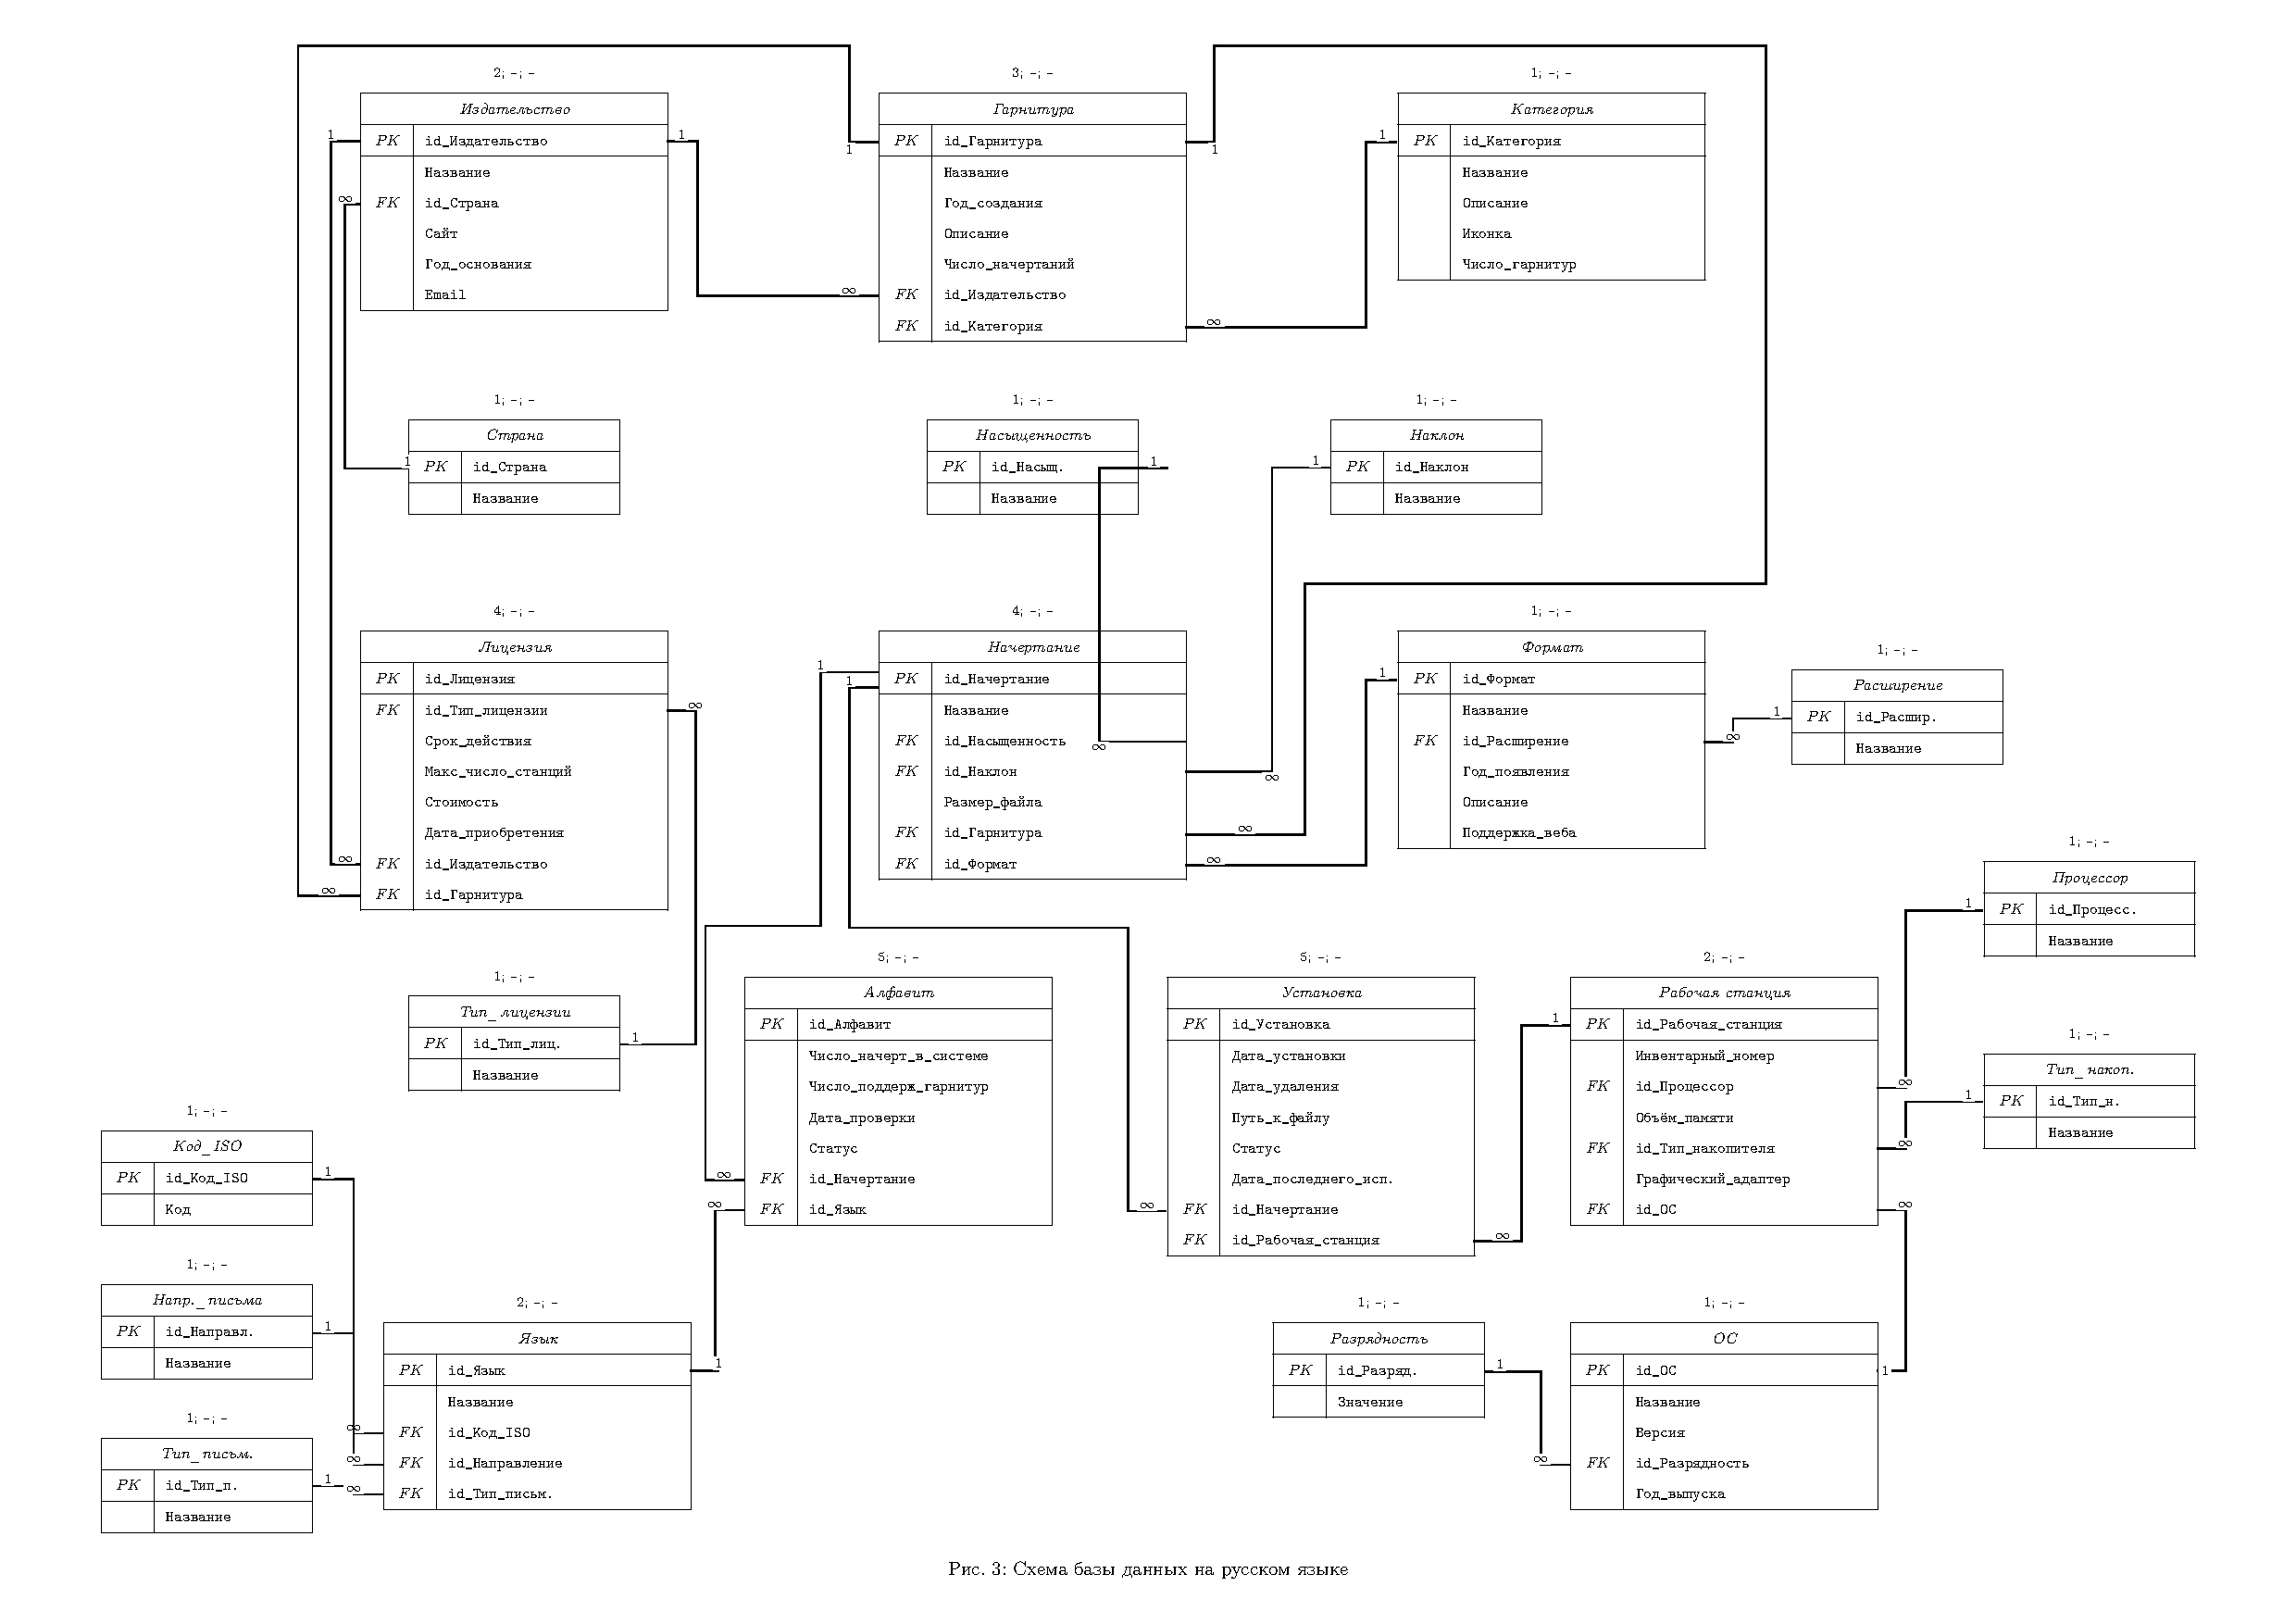
\includepdf[
    pages=1,
    landscape,
    fitpaper,
    pagecommand={\thispagestyle{plain}}
]{tex/graphics/db-schema.pdf}

\clearpage
\refstepcounter{figure}
\label{fig:db-schema-eng}
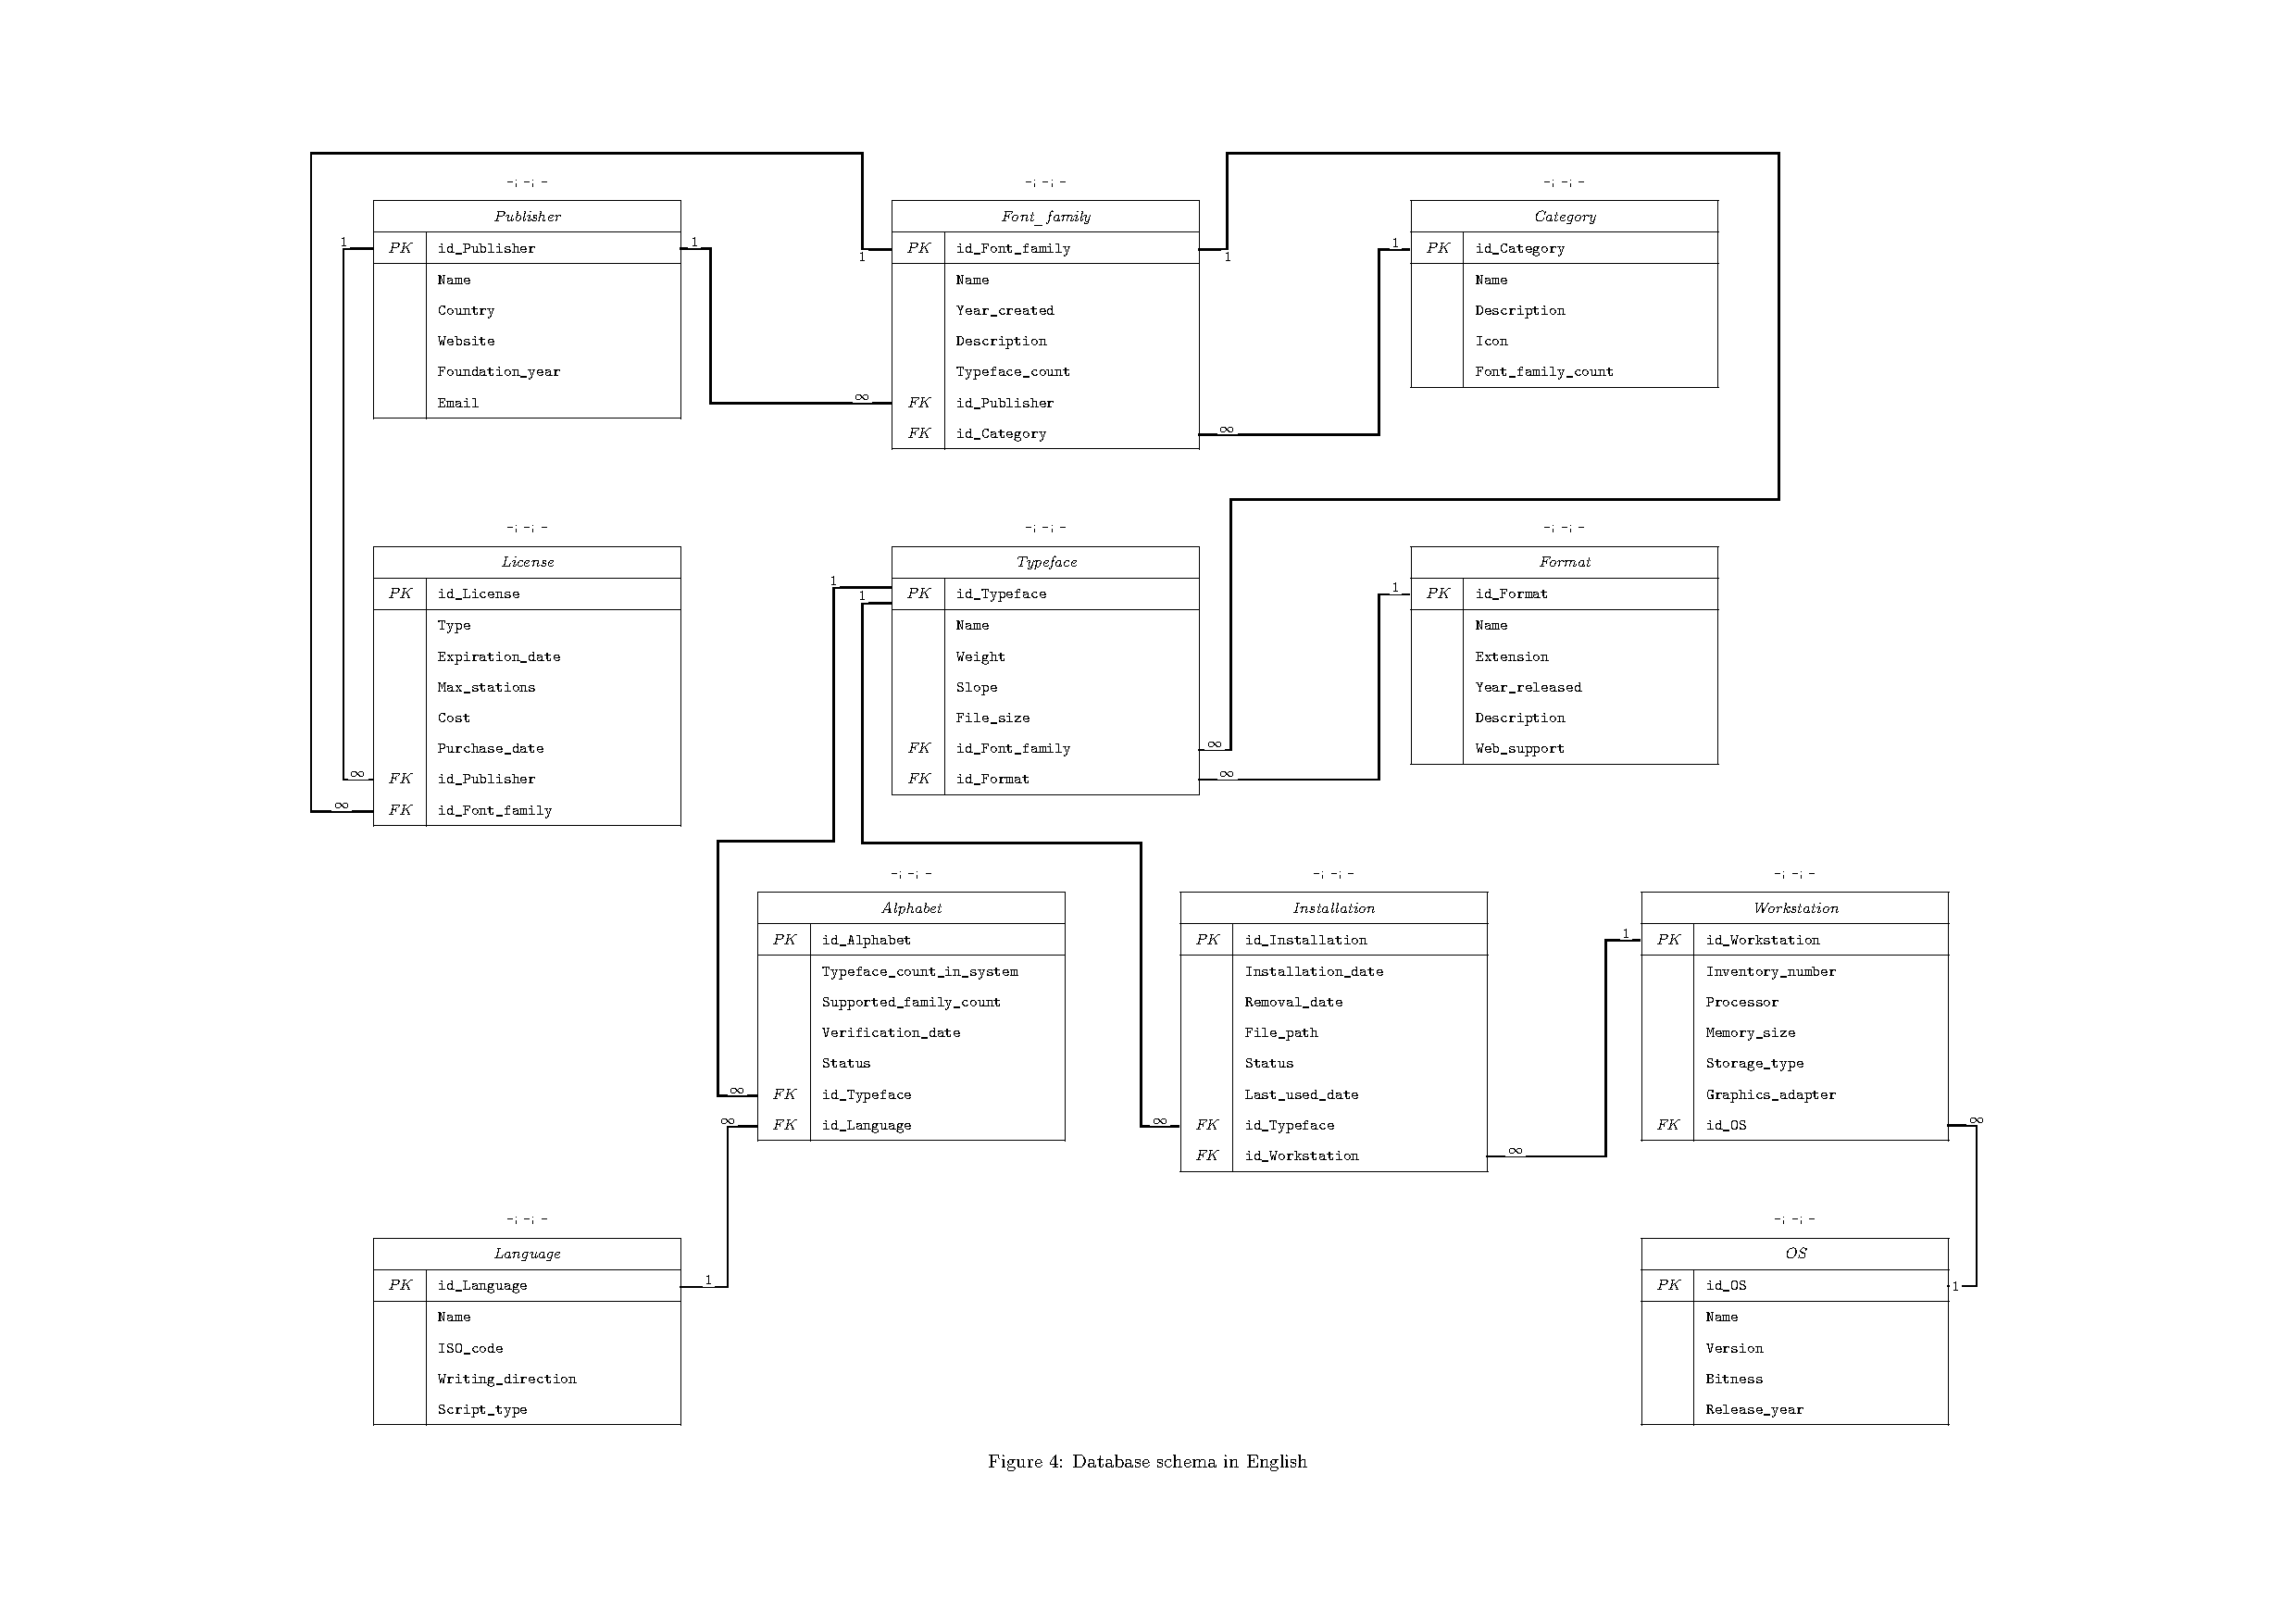
\includepdf[
    pages=1,
    landscape,
    fitpaper,
    pagecommand={\thispagestyle{plain}}
]{tex/graphics/db-schema-eng.pdf}
